\documentclass[a4paper,12pt]{article}
\usepackage{graphicx}
\usepackage[left=30mm, right=30mm, top=30mm, bottom=35mm]{geometry}
\usepackage{amsmath}
\usepackage{siunitx}
\usepackage{fancyhdr}
\usepackage{url}
\pagestyle{fancy}
%-------------------------------------------------------------------------------
\lhead{\textbf{Fall 2020}}
\rhead{\textbf{CE311K Intro to Computer Methods}}
\cfoot{\thepage}
%-------------------------------------------------------------------------------

\begin{document}
\begin{centering}
	\textbf{
		Assignment 01: Iterations and control flow\\
		Assigned: 15th September 2020\\
		Due: 29th September 2020 at 5 PM\\
	}
\end{centering}


Note: Please upload your solution as an ipynb and pdf file to the Canvas page.

\vspace{1em}
 
 The purpose of this assignment is to develop your skills in writing iterations (for) and control flow (if/else).
 
\begin{enumerate}
	\item Write a python code to calculate the sum of first $n$ elements for the following series. Use $n = 15$.
	\begin{enumerate}
		\item Maclaurin series for $\sin(x)$. 
		\begin{equation*}
		x - \frac{x^3}{3!} + \frac{x^5}{5!} - \dots
		\end{equation*}
		for $x = 2.5$. Check your result using \verb|math.sin(x)|.	Hint. To calculate the factorial of a number use the inbuilt function in \verb|math| module \verb|math.factorial(x)|
		\item For $a = 9$ and $r = 1/3$, evaluate the geometric series for the first $n$ terms:
		\begin{equation*}
		a + ar + ar^2 + ar^3 + \dots + ar^{n - 1}
		\end{equation*}
		Check your solution using the geometric series formula:
		\begin{equation*}
			\sum_{k = 0}^{n - 1} ar^k = a \left(\frac{1 -r^n}{1-r}\right)
		\end{equation*}
		
	\end{enumerate}


	
	\item Using control flow  statements write a code that tests the location of a given point $P(x_p, y_p)$ with respect to an annular ring of inner radius $R_i$ and outer radius $R_o$ centered at point $C (x_c, y_c)$ and report if the point lies:
	\begin{enumerate}
		\item inside the annulus
		\item on the annulus
		\item beyond the outer radius
		\item within the inner radius
	\end{enumerate}
	 Test your code for the following annular ring with its center located at $(x_c, y_c) = (2.0, 3.0)$ and the outer radius is 2.0 and inner radius is 1.0. Test for all possible locations of point $P$ (inside, outside, and on either
	 of the two circles).
	 
	\begin{figure}[ht]
	 	\centering
	 	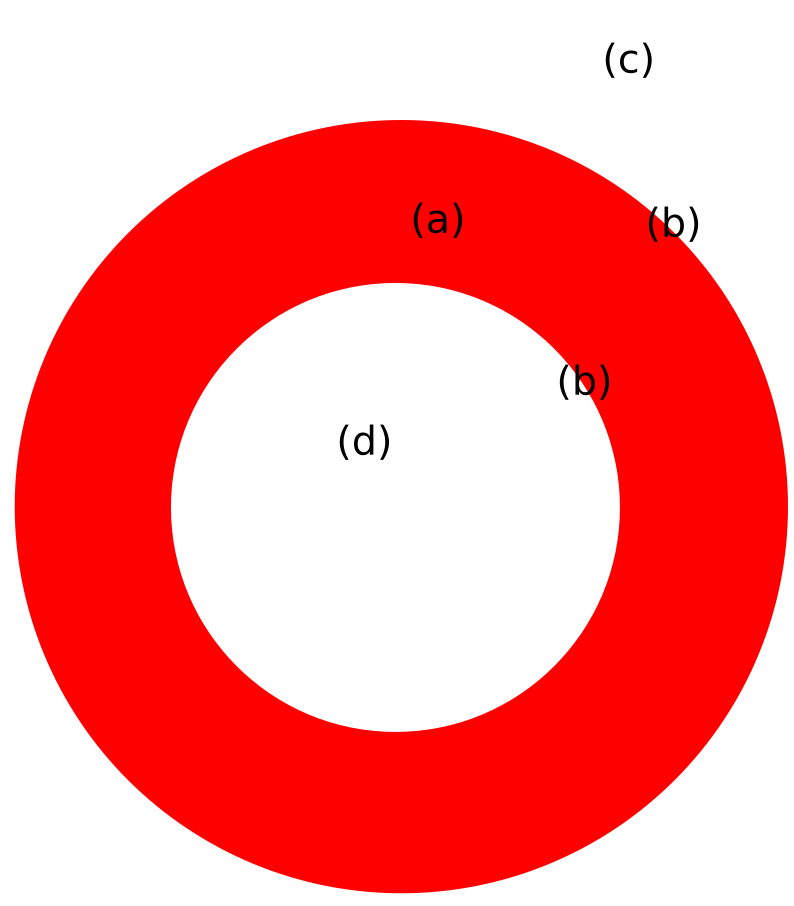
\includegraphics[width=0.3\textwidth]{annulus.png}
	 	\caption{Q2: Annulus}
	 \end{figure}
 
 	\clearpage
	
	\item A simply supported beam of length 20 feet is supporting a uniformly distributed load $q$ of 4000 lb/ft to half its length as shown below. Write a Python code using conditional statements (if/else) to compute the deflection at any location $x$ along the length of the beam.

	\begin{figure}[ht]
		\centering
		\includegraphics[width=0.6\textwidth]{ss-beam.png}
	\end{figure}

	For the given loading, the deflection $\delta(x)$ is:
	
	\begin{equation*}
		\delta(x) = \frac{q x}{384EI}(9L^3 - 24Lx^2 + 16x^3) \qquad 0 \le x \le \frac{L}{2}
	\end{equation*}
	
	and 

	\begin{equation*}
	\delta(x) = \frac{q L}{384EI}(8x^3 - 24Lx^2 + 17L^2x -L^3) \qquad \frac{L}{2} \le x \le L
	\end{equation*}
	
	Note that $x < 0$ and $x > L$ are invalid locations. Use the following values for the various parameters involved in the above expressions:
	
	\begin{align*}
		q & = 4000 ~lb/ft\\
		L & = 20 ~ft\\
		EI & = 1.2e8 ~lb.ft^2
	\end{align*}
	
	Using these values, obtain the deflection at 3 locations: $x = L/4, L/2, 3L/4$.
	
	\item Modify the above code using a for-loop to plot the displacement of the beam along its length. Plot the displacement profile when calculating $x$ at every $0.5, 1, 2$ and $5$ feet (4 different plots).
\end{enumerate}

\end{document}

